\documentclass{beamer}

\usepackage[utf8]{inputenc}
\usepackage{graphicx}
\usepackage{appendixnumberbeamer}
\usepackage{amsmath}

\usetheme{CambridgeUS}
\usecolortheme{beaver}

\setbeamertemplate{navigation symbols}{}

\title[ProbEmbed]{Learning Embeddings with Dirichlet Processes and Heavy Tails}
\author{Adith -- Chenhao -- Moontae}
\institute{Cornell}
\date{September 19th, 2014}

\begin{document}
\begin{frame}
\titlepage
\end{frame}

\begin{frame}{Learning embeddings}
  \begin{itemize}
    \item Mapping discrete atoms (words/phrases) into a continuous space
    \item To achieve a distributed and dense representation \cite{Hinton} 
    \item Useful representation for several NLP tasks \cite{Turian}
  \end{itemize}
 \vspace{-10px}
\begin{figure}[h!]
  \caption{Discovering implicit relationships between words \cite{CBOW}}
  \centering
    %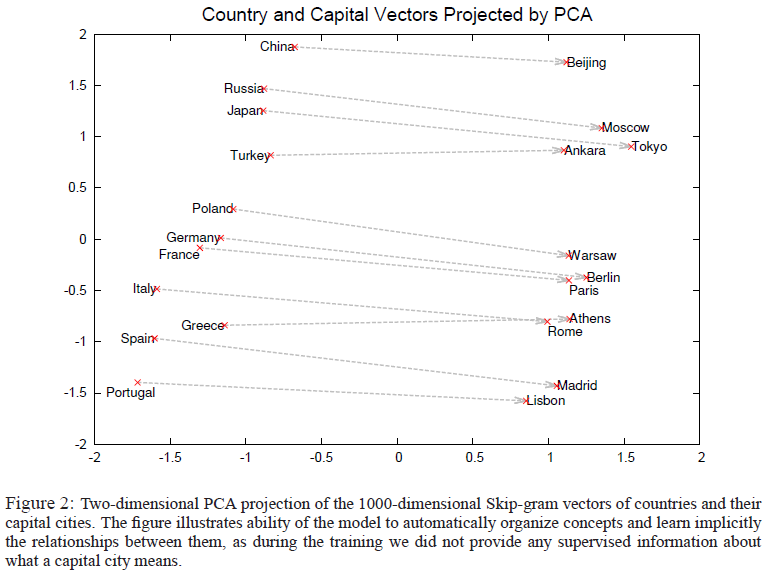
\includegraphics[trim = 0mm 80mm 0mm 0mm, width=0.6\textwidth]{CBOW.png}
    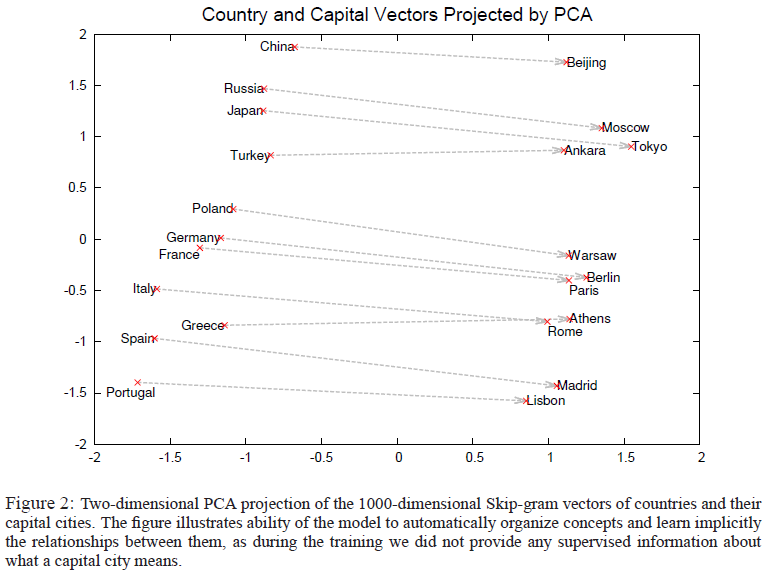
\includegraphics[width=0.5\textwidth]{CBOW.png}
\end{figure}
%\vspace{40px}
\end{frame}

\begin{frame}{Learning embeddings}
\begin{figure}[h!]
  \caption{Discovering concept clusters \cite{Socher}}
  \centering
    %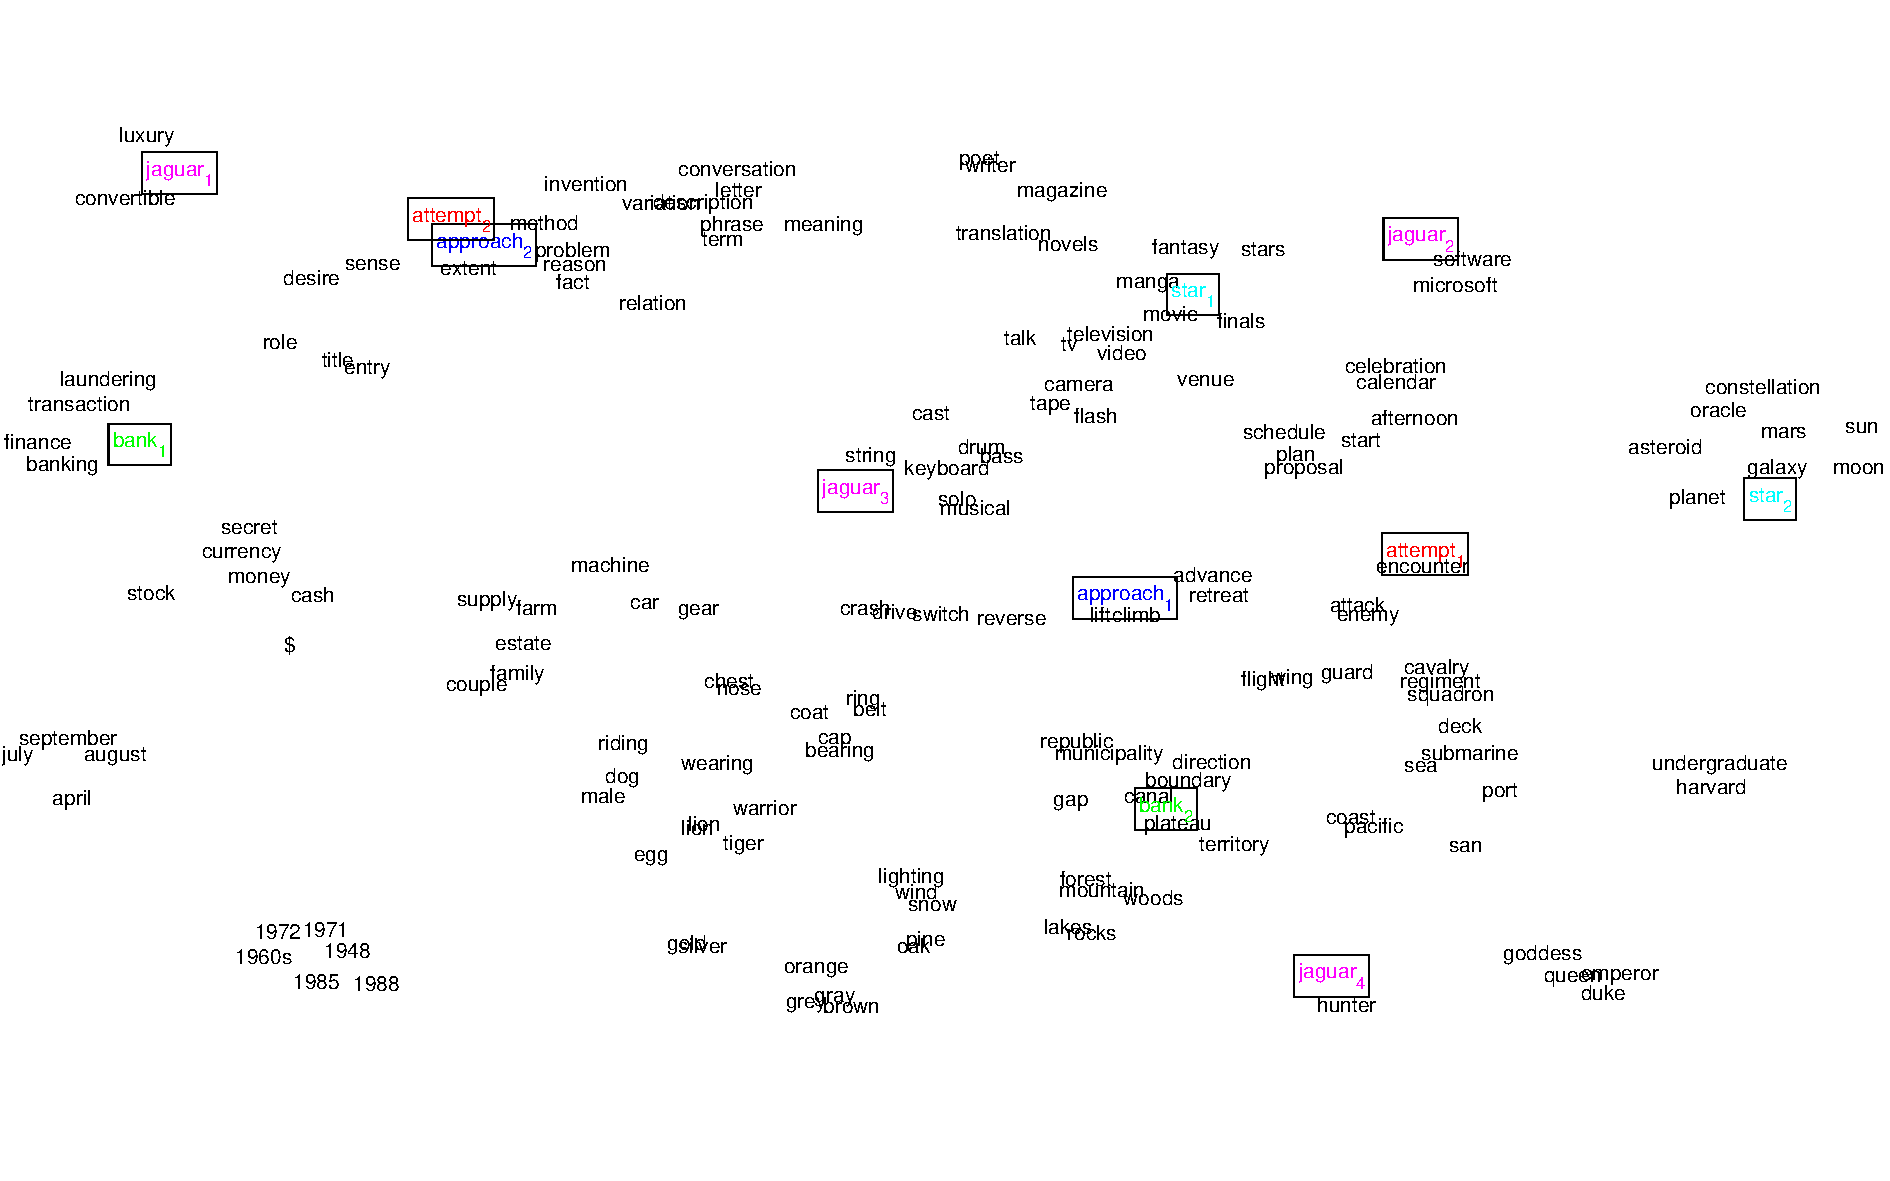
\includegraphics[trim = 0mm 0mm 0mm 1mm, width=0.9\textwidth]{MultipleVectorWordEmbedding.pdf}
    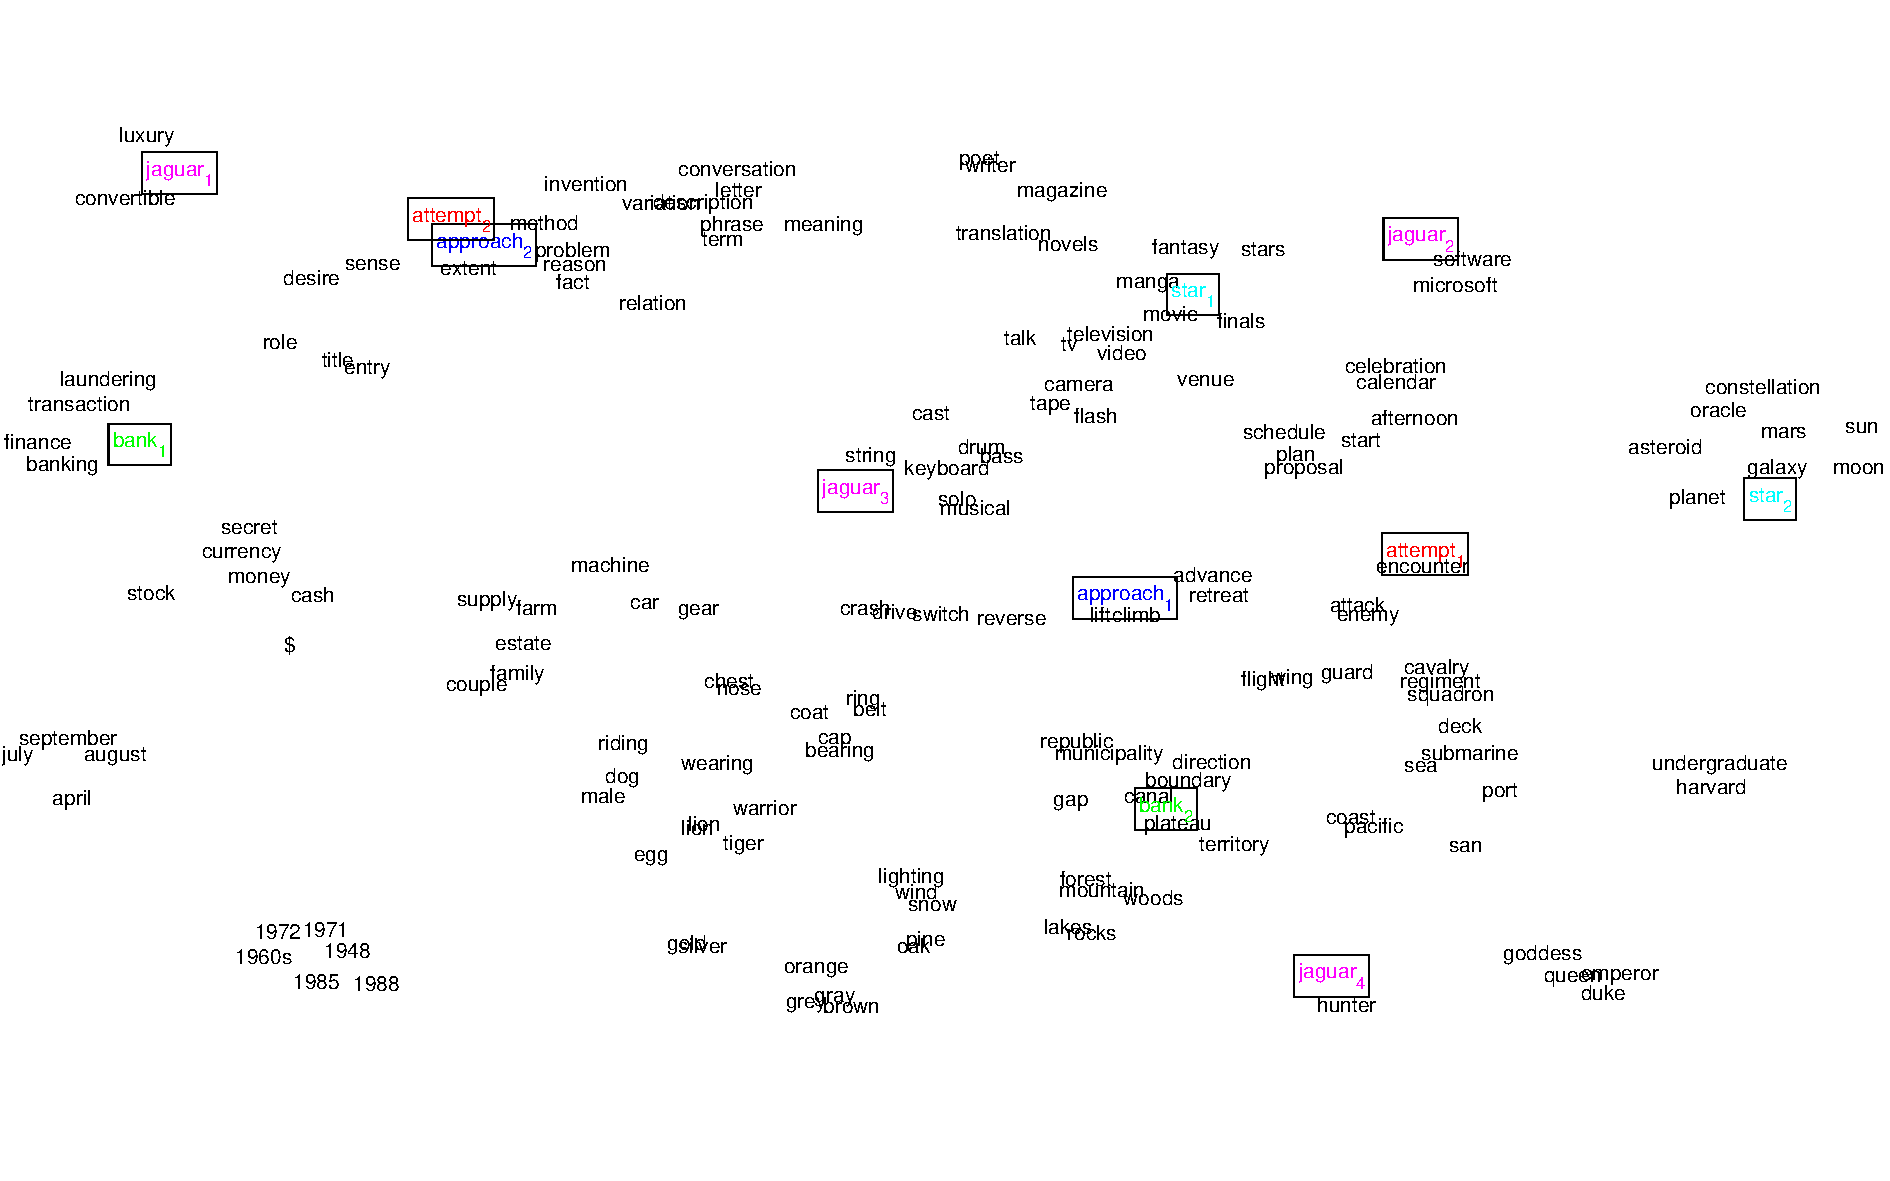
\includegraphics[width=0.7\textwidth]{MultipleVectorWordEmbedding.pdf}
\end{figure}
\begin{itemize}
    \item A typical way to validate embedding quality
\end{itemize}
\end{frame}

\begin{frame}{An incomplete and utter history of word embeddings}
  \begin{itemize}
    \item Distributional clustering \cite{Lillian}
    \item SENNA \cite{Collobert}
    \item WordReprs \cite{Turian}
    \item NCE \cite{Mnih}
    \item Multi-prototype \cite{Socher}
    \item CBOW/Skip-gram \cite{CBOW}
    \item Matrix factorization approaches \cite{Moitra}
    \item Generative Topic Models \cite{LDA}
  \end{itemize}
\end{frame}

\begin{frame}{Goal}
A generative model of word embeddings that
\begin{itemize}
\item Takes as input $D$: all observed text
\item Outputs an embedding $X$: words situated in a vector space
\item such that the embeddings cluster around concepts
\item distances/directions in the embedding space directly model data distribution
\item which is scalable to learn
\item and also recover good performance of existing embeddings in other settings
\end{itemize}
\end{frame}

\begin{frame}{Why generative models?}
  \begin{itemize}
    \item Learning problem is well specified in a principled way
    \item Modular models for adding complexity/assumptions
    \item Embedding quality aligned with learning objective
    \item Diagnostics to verify model assumptions
  \end{itemize}
\end{frame}

\begin{frame}{Formal specification}
  \begin{block}{Bayesian framework}
    $\Pr(X)$: prior\\
    $\Pr(D \mid X)$: likelihood
  \end{block}
  \begin{block}{Learning problem}
	$X^* = argmax_{ X } \Pr(X \mid D) = argmax_{ X } \Pr(X) \cdot \Pr(D \mid X)$
  \end{block}
  \begin{block}{Evaluation}
	$\Pr(D_{heldout} \mid X^*)$\\
    Are ground-truth clusters preserved in embedding?\\
    etc.
  \end{block}
  \pause
  \begin{alertblock}{Question}
	What other evaluations should we do \& who to compare against?
  \end{alertblock}
\end{frame}

\begin{frame}{Example: Logistic Markov Embedding}
  \begin{block}{Embedding songs from playlists \cite{LME}}
  	\begin{itemize}
    		\item $D: $ Playlists $p = s_1 \dots s_{|p|}$, first order markov chains
    		\item $s_i \mapsto X_i \overset{iid}{\sim} \mathcal{N}(\vec{0}, \lambda^2 \mathcal{I})$\\
    		\item $\Pr(s_j \mid s_i ; X) \propto expo(-\| X_i - X_j \|^2)$
    \end{itemize}
    \end{block}
    \begin{block}{Learning}
    		\begin{align*}
    		argmax_{ X } \prod_p \prod_{i=1}^{|p|-1} \Pr(s_{i+1} \mid s_i ; X) &\cdot \prod_i \Pr(X_i) \\
		\equiv argmin_{ X } -\sum_i \sum_j \#(s_i \rightarrow s_j) \cdot \log \Pr(s_j \mid s_i ; X) &+ \frac{1}{2 \lambda^2} \sum_i \| X_i \|^2
		\end{align*}
    \end{block}
\end{frame}

\begin{frame}{Logistic vs. Heavy-Tailed Dirichlet Process Markov Embedding}
\begin{columns}[c]
\column{5.5cm}
\begin{figure}
  \caption{Logistic Markov Embedding on \emph{YES-small} dataset \cite{LME}}
    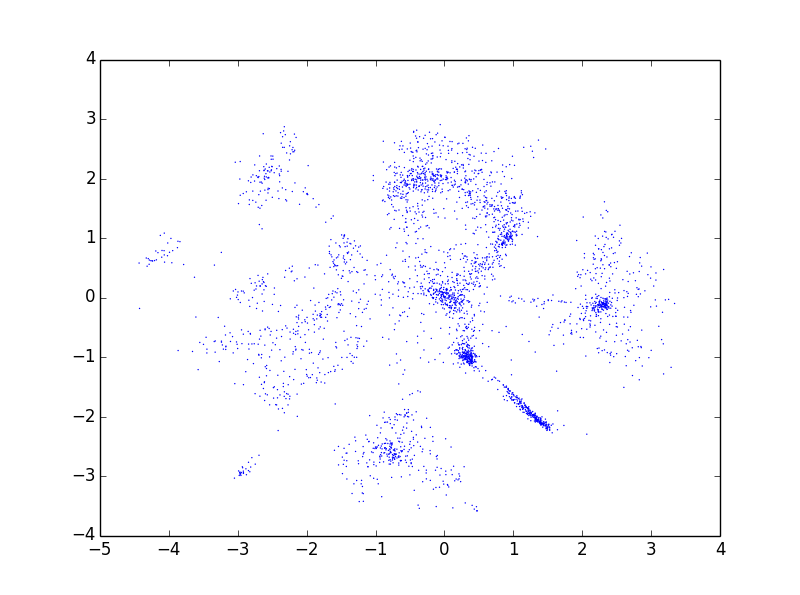
\includegraphics[width=0.95\textwidth]{LME.png}
\end{figure}
\column{5.5cm}
\pause
\begin{figure}
  \caption{Heavy-tailed Dirichlet Process Embedding}
  \vspace{15px}
    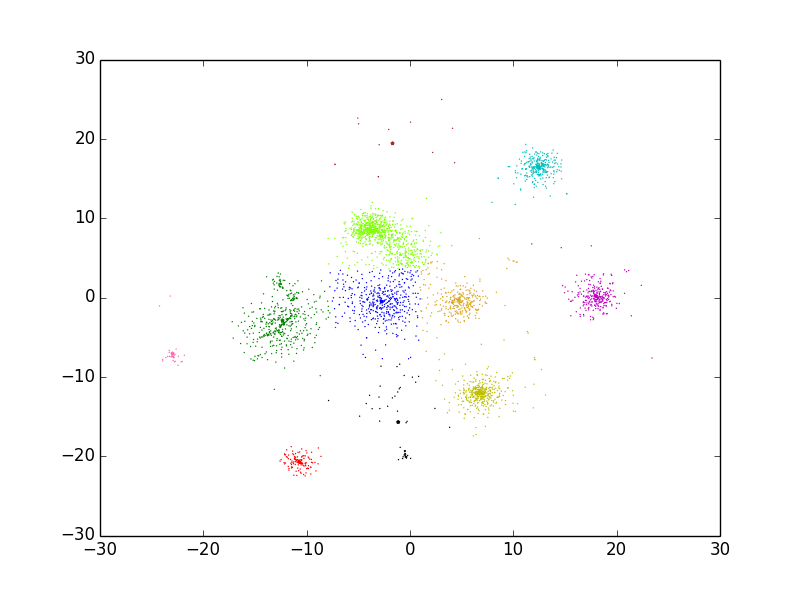
\includegraphics[trim=0mm 2mm 0mm 0mm, width=0.95\textwidth]{ProbEmbed.png}
\end{figure}
\end{columns}
\end{frame}

\begin{frame}{Why use heavy-tailed distribution?}
  \begin{itemize}
    \item Heavy-tails can properly model many small probabilities
    \item Avoids ``crowding problem'' (curse of dimensionality)
    \item Not enough space that models high-dimensional points in low dimensional space
  \end{itemize}
\end{frame}

\begin{frame}{Heavy-Tailed Dirichlet Process Markov Embedding}
   \begin{block}{Heavy tails}
    $\Pr(s_j \mid s_i ; X) \propto \frac{1}{1 + \| X_i - X_j \|^2}$
   \end{block}
  \begin{block}{DPMeans \cite{DPMeans}}
  \begin{itemize}
	\item $K, z_{1 \colon N} \sim \mathcal{CRP}(\theta)$
	\item $\mu_{1 \colon K} \overset{iid}{\sim} \mathcal{N}(\vec{0}, \rho^2 \mathcal{I})$
	\item $X_i \sim \mathcal{N}(\mu_{z_i}, \sigma^2 \mathcal{I})$
	\item Set $\theta = \exp(\frac{-\lambda^2}{2 \sigma^2})$, and take $\lim \sigma^2 \rightarrow 0$
  \end{itemize}
  \end{block}
  \begin{block}{Small variance MAP Clustering}
	$argmin_{\mu, z, K} -2 \sigma^2 \log \Pr(z, \mu, X) \sim \sum_{k=1}^K \sum_{i : z_i = k} \| X_i - \mu_k \|^2 + \lambda^2 \cdot (K - 1)$
  \end{block}
\end{frame}

\begin{frame}{Learning clustered word embeddings}
  \begin{block}{Empirical replacement probability}
  \begin{align*}
   \hat{\Pr}(w_j \mid w_i ; D) &= \sum_{\text{contexts } c} \hat{\Pr}(w_j, c \mid w_i ; D)\\
    & = \sum_c \hat{\Pr}(w_j \mid c ; D) \cdot \hat{\Pr}(c \mid w_i ; D) \\
    & = \sum_c \frac{\#(c, w_j)}{\#(c)} \cdot \frac{\#(c, w_i)}{\#(w_i)}
  \end{align*}
  \end{block}
  \begin{block}{Modeling replacement probability}
          $\Pr(w_j \mid w_i ; X) \propto \frac{1}{1 + \| X_i - X_j \|^2}$
  \end{block}
  \pause
  \begin{alertblock}{Question}
	Should we model replacement probability or co-occurrence (or other)?
  \end{alertblock}
\end{frame}

\begin{frame}{Learning clustered word embeddings}
  \begin{block}{Co-occurrence matrix $C$}
  \begin{align*}
   \hat{\Pr}(w_j \mid w_i ; D) &= \hat{\Pr}(w_j, w_i ; D) / \hat{\Pr}(w_i ; D)\\                             
    & = \frac{\hat{\Pr}(w_j, w_i ; D)}{\sum_{j'} \hat{\Pr}(w_j', w_i ; D)} = \frac{C_{ji}}{\sum_{j'}C_{j'i}}                        
  \end{align*}
  \end{block}
  \pause
  \begin{alertblock}{Problem}
    \begin{itemize}
       \item Could be very sparse
       \item Less occurring words are rewarded during normalization process
       \item Unclear what the correct diagonal entries are
       \item Need to satisfy certain algebraic structures
    \end{itemize}
  \end{alertblock}
\end{frame}




\begin{frame}{Learning clustered word embeddings}
  \begin{block}{Objective: Minimize KL-Divergence}
    \begin{align*}
    argmin_{X, \mu, z, K}  - \sum_i \sum_j & \hat{\Pr}(w_j \mid w_i ; D) \log \Pr(w_j \mid w_i ; X) \\
    &+ \frac{1}{2 \sigma^2} \{ \sum_i \| X_i - \mu_{z_i} \|^2 + \lambda^2 \cdot (K - 1) \} 
    \end{align*}
  \end{block}
  \pause
  \begin{alertblock}{Question}
	This objective is not generative. Can we recover generative likelihood?
  \end{alertblock}
\end{frame}

\begin{frame}{Questions?}
  \begin{itemize}
    \item This objective is not generative. Can we recover generative likelihood?
    \item Can we actually evaluate based on generative story?
    \item What other evaluations should we do \& who to compare with?
    	\item Should we model replacement probability or co-occurrence (or other)?
  \end{itemize}
\end{frame}

\appendix

\begin{frame}[allowframebreaks]{References}
  \bibliographystyle{apalike}
  \bibliography{ProbEmbed}
\end{frame}

\end{document}